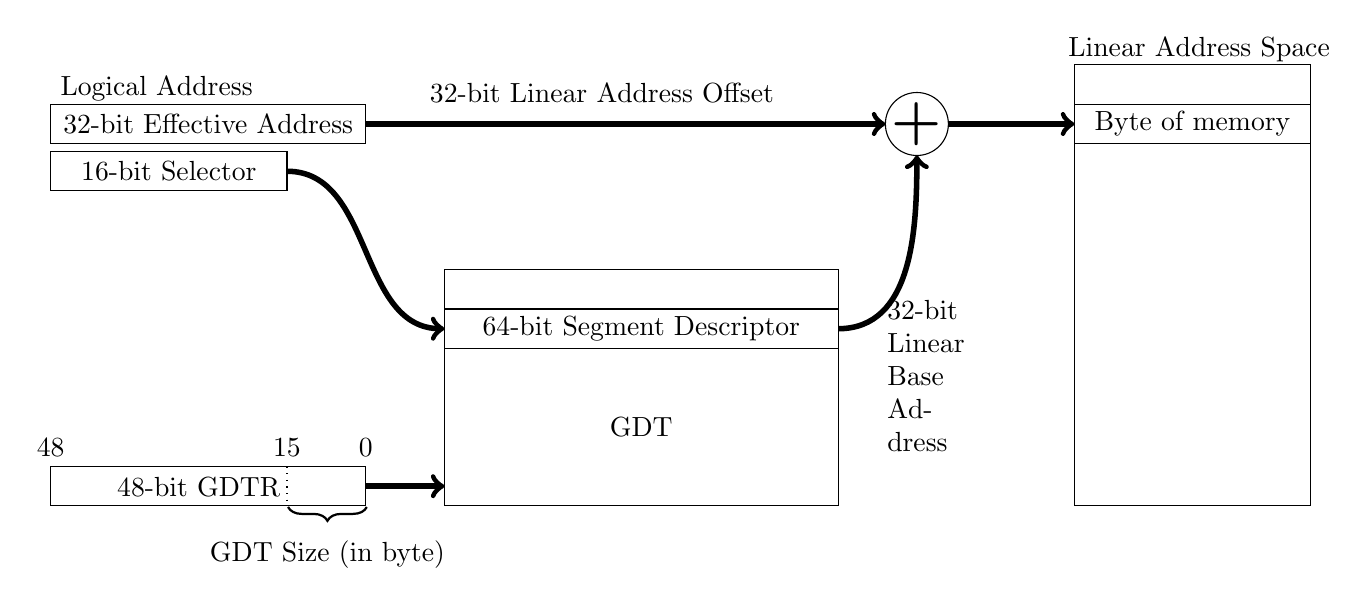
\begin{tikzpicture}
\draw (0,0) rectangle (4,0.5) node [pos=0.47] {48-bit GDTR};
\draw [thick,decorate,decoration={brace,amplitude=5pt,mirror},xshift=0.4pt,yshift=-0.4pt](3,0) -- (4,0) node[black,midway,yshift=-0.6cm] {GDT Size (in byte)};
\draw node at (0,0.5) [above] {48};
\draw node at (4,0.5) [above] {0};
\draw[dotted] (3,0.5) node [above] {15} -- (3,0);

\draw (5,0) rectangle (10,2) node [pos=0.5] {GDT};
\draw (5,2) rectangle (10,2.5) node [pos=0.5] {64-bit Segment Descriptor};
\draw (5,2.5) rectangle (10,3);

\draw (0,4) rectangle (3,4.5) node [pos=0.5] {16-bit Selector};
\draw (0,4.6) rectangle (4,5.1) node [pos=0.5] {32-bit Effective Address};
\draw node at (0,5.3) [above, right] {Logical Address} ;

\draw[->, line width = 2pt] [out = 0] (3,4.25) to [in = 180] (5,2.25);
\draw[->, line width = 2pt] [out = 0] (4,0.25) to [in = 180] (5,0.25);

\draw (11,4.85) circle (0.4) node {\textbf{\huge +}};
\draw[->, line width = 2pt] [out = 0] (4,4.85) to [in = 180] (10.6,4.85) ;
\draw node at (7,5) [above] {32-bit Linear Address Offset} ;
\draw[->, line width = 2pt] [out = 0] (10,2.25) to [in = -90] (11,4.45);
\draw node at (10.5,1.65) [right,text width=1.2cm] {32-bit Linear Base Address} ;

\draw (13,0) rectangle (16,4.6);
\draw (13,4.6) rectangle (16,5.1) node [pos=0.5] {Byte of memory};
\draw (13,5.1) rectangle (16,5.6);
\draw node at (12.8,5.8) [above, right] {Linear Address Space} ;
\draw[->, line width = 2pt] [out = 0] (11.4,4.85) to [in = 180] (13,4.85);
\end{tikzpicture}